 
   %judul bisa diketik ulang
  \setstretch{1}%\small
  \begin{center}
      \textbf{\large \Title}\\
      \bigskip 
  \end{center}
  
  
  
  %Nama authors
   \begin{center}
     \bf \Author$^1$, Pemb 1 tanpa gelar$^2$, Pemb 2 tanpa gelar$^3$, Pemb 3 tanpa gelar$^4$ 
  \end{center}
  
  
  %Afiliasi dan email
   \begin{center}
     $^{1,2,3}$Fakultas Informatika, Universitas Telkom, Bandung\\
$^4$Divisi Digital Service PT Telekomunikasi Indonesia\\
$^1$mhs@students.telkomuniversity.ac.id, $^2$pembimbing1@telkomuniversity.ac.id,\\ $^3$pembimbing2@telkomuniversity.ac.id, $^4$pembimbingluar@telkom.co.id 
  \end{center}
  
   
 %%% Abstrak Indonesia %%%%%%%%%%  
   
{\bf \parindent0pt \noindent\rule{\textwidth}{1pt}
Abstrak

Dokumen ini merupakan panduan penulisan jurnal Tugas Akhir (TA) di lingkungan Fakultas Informatika Universitas Telkom. Meskipun demikian, dimungkinan/dipersilahkan untuk pembimbing TA menggunakan struktur penulisan yang tidak sama persis dengan yang ada di dokumen ini. Panjang abstrak tidak lebih dari 200 kata dan diketik dalam ukuran huruf 10 pts. TA sebagai salah satu sarana latihan penulisan akademik dan memperjelas tulisan, abstrak dibagi menjadi empat paragraf atau sub-bagian. Setiap sub bagian bisa diberi judul yang digaris bawahi. Abstrak berisi apa, mengapa, bagaimana, dan hasil utama (kesimpulan).\\

\underline{\textit{Apa permasalahan pada topik}}. Yang juga menjelaskan latar belakang permasalahan topik. Sebaiknya tuliskan juga apa masukan dan keluaran secara sangat singkat. \\

\underline{\textit{Mengapa topik menarik atau penting}}. Sebisa mungkin tuliskan contohnya secara sangat singkat. Pada bagian ini sebaiknya ditulis juga \textit{apa masalah/kekurangan yang terjadi unt kondisi saat ini} (gap antara kondisi sekarang dengan yang diharapkan)? \\

\underline{\textit{Bagaimana solusinya}}. Jelaskan secara garis besar sistem solusi yang telah dilakukan. Biasanya penjelasan solusi ini merupakan yang terpanjang pada abstrak. \\

\underline{\textit{Hasil utama}}. Hasil utama dari eksperimen ditulis singkat dua-tiga kalimat. Akan lebih baik (optional), kalau dituliskan secara eksplisit kontribusi yang telah dihasilkan. Kontribusi bisa dituliskan diantara bagian solusi dan hasil eksperimen. \\

Pastikan abstrak pada jurnal TA tidak copas dari abstrak proposal TA. Pada abstrak proposal kadang ada kata \textit{akan}, seperti misalnya \textit{yang akan dilakukan}; sedangkan pada abstrak Jurnal TA tidak ada kata \textit{akan} spt itu. Tidak boleh ada sitasi pada abstrak. Pada abstrak tidak menggunakan penamaan, simbol atau istilah yang teknis, misalnya \textit{minsup} untuk menyatakan nilai support minimal.

 \bigskip
Kata kunci : merupakan kata-kata kunci yang menjelaskan isi tulisan, biasanya bisa diambil dari judul dan abstrak. Maksimal enam buah dan ditulis dengan huruf kecil, kecuali singkatan



%%% Abstrak English %%%%%%%%%%  



\noindent\rule{\textwidth}{1pt}
Abstract

The abstract should state briefly the general aspects of the subject and the main concolusions.  The length of abstract should bo no more than 200 word and  should be typed be with 10 pts.

 \bigskip
Keywords: keyword should be chosen that they best describe the contents of the paper and should be typed in lower-case, except abbreviation. Keyword should be no more than 6 word 

\noindent\rule{\textwidth}{1pt} }
   


%%%%%% isi paper %%%%

\section{Pendahuluan}

Naskah jurnal ditulis di kertas berukuran standar A4 (21 cm $\times$ 29.7 cm) dalam empat sampai delapan halaman. Naskah ditulis dalam format satu spasi. Tambahkan satu spasi untuk setiap antar-bagian (antara judul dan penulis, antara penulis dan abstrak, antara abstrak dan kata kunci, antara sub-bab dan isi). Semua margin atas, margin bawah, margin kiri, dan margin kanan 25 mm. Margin untuk header dan footer 15 mm. Naskah tidak perlu diberi header dan footer. 

Jurnal TA berisi abstrak, pendahuluan, studi terkait (\textit{related works}) atau studi pustaka (\textit{literature review}), sistem yang dibangun,  evaluasi, dan kesimpulan. Setiap bagian Jurnal TA dijelaskan secara rinci di bagian bawah bab ini.
Judul TA dalam kalimat lengkap yang  singkat, spesifik, dan jelas memberi gambaran tentang isi TA. Jika pada judul menyatakan sistem/algoritma/pendekatan yang digunakan, maka pada isi (dimulai pada abstrak) berilah justifikasi mengapa sistem tersebut dipilih.

Untuk nama penulis, tuliskan nama lengkapnya. \textbf{Mahasiswa sebagai penulis pertama (\textit{author})}, sedangan pembimbing sebagai \textit{co-author} (penulis dua dan tiga). Diperkenankan ada penambahan co-author yang namanya tidak tercantum dalam SK TA tetapi memberikan kontribusi terhadap makalah ilmiah tersebut. Jumlah penulis maksimal empat orang. Tuliskan nama dan gelar pembimbing dengan benar. Untuk institusi bagi mahasiswa dan dosen pembimbing dari Fakultas Informatika dituliskan afiliasi ‘Fakultas Informatika’ (bukan nama program studi). Untuk email, tuliskan email institusi untuk mahasiswa dan dosen yaitu @student.telkomuniversity.ac.id dan @telkomuniversity.ac.id. Sedangkan untuk pembimbing dari luar kampus dituliskan afiliasi dan alamat email sesuai institusi yang bersangkutan.

Isi bagian Pendahuluan pada prinsipnya merupakan penjelasan lebih detil dari abstrak (utamanya menerangkan \textit{apa} dan \textit{mengapa}), dengan beberapa revisi (tidak \textit{copy paste} dari abstrak).  Isi Pendahuluan terutama menjelaskan latar belakang, penjelasan/identifikasi topik/masalah dan batasannya, tujuan, dan metode penelitian. Isi bagian Pendahuluan diakhiri dengan sistematika/organisasi penulisan. Berbeda dengan bagian Abstrak, pada bagian Pendahuluan ini penjelasan tentang \textit{bagaimana} solusi yang dilakukan, tidak terdapat pada bagian Pendahuluan, namun dijelaskan pada bagian tersendiri.

Panjang bagian Pendahuluan pada jurnal TA antara satu setengah hingga dua halaman untuk jurnal delapan halaman. Beberapa bagian Pendahuluan pada jurnal TA diambil dari Bab Pendahuluan pada proposal TA. Namun, penjelasan-penjelasan pada Bab Pendahuluan proposal TA tersebut perlu diupdate dulu sebelum digunakan. Perbedaan antara bagian pendahuluan dengan yang ada pada proposal TA adalah sebagai berikut. Pertama, Pendahuluan pada jurnal TA lebih pendek dibandingkan yang ada pada proposal. Kedua, pada proposal ada bagian Rencana Kegiatan, sedangkan pada jurnal TA menjelaskan metodologi penyelesaian masalah. Ketiga, pada jurnal TA ada tambahan  sistematika/organisasi tulisan. Keempat, pada jurnal TA tidak ada jadwal kegiatan.

Pada banyak jurnal untuk penelitian, bagian Pendahuluan hanya terdiri dari satu bagian (\textit{section}) tidak dibagi bagi lagi menjadi sub-bagian. Namun, sebagaimana pada Abstrak jurnal TA, sebagai salah satu sarana latihan penulisan akademik dan memperjelas tulisan, bagian Pendahuluan pada jurnal TA dibagi menjadi beberapa paragraf atau sub-bagian. Setiap sub bagian bisa diberi judul yang dengan font tebal atau digaris bawahi. Sebagai contoh berikut ini.\\

\noindent\textbf{Latar Belakang}

Pada sub-bagian ini tuliskan secara singkat tuliskan apa topik yang dikerjakan (mirip dengan yang teklah ditulis di abstrak). Nanti permasalahan akan dijelaskan secara lebih detil di sub-bagian Perumusan Masalah. Kembangkan penjelasan dengan membuat secara lebih detil yang sudah ada di abstrak tentang dua hal berikut. Pertama, mengapa topik yang dipilih menarik dan/atau penting dan/atau sesuai untuk dikerjakan sebagai TA. Kedua, bagaimana dengan kekurangan kondisi saat ini unt topik tersebut (gap/kesenjangan antara kondisi saat ini dengan kondisi yang diharapkan).

Jika pada judul TA dituliskan menggunakan suatu pendekatan/metode/algoritma tertentu, jelaskan secara singkat alasan pemilihannya.\\

\noindent\textbf{Topik dan Batasannya}

Sub-bagian ini bisa juga dinamakan Perumusan Masalah atau Identifikasi Masalah. Untuk nama dalam Bahasa Inggris nama yang populer adalah \textit{Problem Statement} atau \textit{Problem Identification.}

Sub-bagian ini mempunyai fungsi sebagai penjelasan tentang topik TA yaitu apa isu/permasalahan yang akan dikerjakan. Untuk lebih memperjelas bisa juga disampaikan definisi atau pengertian. Penyampaian definisi dan penjelasan pada sub-bagian ini sebaiknya dilakukan dalam tulisan naratif dan informal (tanpa formula matematis) apa topik permasalahan yang telah dikerjakan untuk TA. Untuk mempermudah dalam menuliskan sub-bagian ini, dapat dipandang membuat penjelasan kata-kata kunci (pada abstrak) dan judul TA. Dengan penjelasan di sub-bagian ini, maka topiknya menjadi jelas bagi pembaca. Kalau digambarkan dalam sebuah algoritma, maka salah satu materi utama pada sub-bagian ini menjelaskan apa input dan output dari algoritma tersebut. Oleh karena itu, sangat dianjurkan untuk menerangkan apa input dan output, serta sebuah contoh kasusnya secara sangat singkat.

Sebutkan batasan pekerjaan yang ada. Batasan adalah kondisi-kondisi penyederhaan permasalahan, sehingga membuat pekerjaan semakin jauh dari ideal. Batasan masalah berisi pembatasan-pembatasan permasalahan agar menjadi lebih sederhana sehingga bisa/layak dikerjakan sebagai TA yang empat SKS dalam satu semester. Batasan diperlukan karena keterbatasan sumber daya saat pengerjaa TA, misalnya keterbatasan waktu pengerjaan yang hanya satu semester, keterbatasan data pendukung (misalnya tidak tersedianya korpus pengetahuan yang diperlukan) dan keterbatas kemampuan (misalnya untuk implementasi algoritma yang kompleks, dalam implementasinya diimplementasikan bentuk penyederhanaan). Salah satu ciri batasan yang bisa dipakai adalah bila bisa digunakan pada sub-bagian Saran (pada bagian Kesimpulan) agar TA berikutnya melonggarkan atau meniadakan batasan tersebut. Penyederhanaan yang dituliskan untuk batasan, antara lain meliputi data yang ditangani/digunakan, misalnya  jumlah data yang digunakan relatif sedikit, dan proses yang dikerjakan, misalnya ada satu subproses yang dikerjakan secara manual. Sebaiknya setiap batasan diberi alasan, misalnya jumlah data yang digunakan hanya 500 buah (relatif sedikit dibandingkan banyak penilitian unt topik sejenis) karena keterbatasan kemampuan komputer yang tersedia. Contoh lain, misalnya proses pelabelan peran semantik pada kalimat Bahasa Indonesia dilakukan secara manual, karena saat ini belum ditemukan alat bantu otomatis unt pelabelan peran semantik untuk Bahasa Indonesia yang efektif. Contoh batasan masalah yang tidak perlu misalnya sudah jelas tercerminkan pada judul.\\

\noindent\textbf{Tujuan}

Sub-bagian Tujuan ini menerangkan kondisi apa yang hendak dicapai atau pertanyaan yang hendak dicari jawabannya. Sebisa mungkin tuliskan kondisi yang hendak dicapai yang terukur (bisa diukur dengan metrik evaluasi yang ditetapkan).  
Penulisan diupayakan dalam bentuk narasi (bukan berupa poin-poin).

Tujuan-tujuan yang ditetapkan menjadi bahan untuk menentukan skenario eksperimen yang dilakukan. atau dengan kata lain eksperimen dilakukan sesuai dengan tujuannya. Kemudian, kesimpulan pada jurnal TA harus selaras dengan tujuan. Hal ini bisa diilustrasikan pada Gambar 1 atau Tabel 1.
\begin{figure}[h!]
\centering
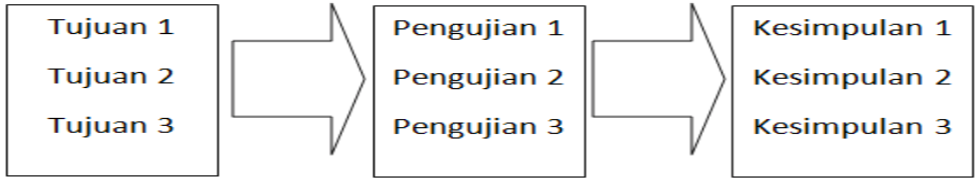
\includegraphics[scale=0.30]{Tujuan.png}
\caption{\textbf{Keterkaitan antara tujuan, pengujian dan kesimpulan}}
\label{fig:tujuan}
\end{figure}

\begin{table}[h!]
\caption{\textbf{Keterkaitan antara tujuan, pengujian dan kesimpulan}}
\label{table:1}%\bigskip
\centering
\begin{tabular}{| c | c  | c | c |} 
 \hline
 \textbf{No} & \textbf{Tujuan} & \textbf{Pengujian} & \textbf{Kesimpulan} \\ [0.5ex] 
 \hline
 1 & Tujuan 1 & Pengujian 1 & Kesimpulan 1 \\ 
 2 & Tujuan 2 & Pengujian 2 & Kesimpulan 2 \\ 
 3 & Tujuan 3 & Pengujian 3 & Kesimpulan 3 \\  [1ex] 
 \hline
\end{tabular}

\end{table}

\noindent \textbf{Organisasi Tulisan}

Pada sub-bagian ini dituliskan bagian-bagian selanjutnya (setelah Pendahuluan) pada jurnal TA ini, disertai penjelasan sangat singkat.

\section{Studi Terkait}
Bagian ini berisi teori/studi/literatur yang mendukung (terkait erat) dengan topik TA yang dikerjakan. Bagian ini bisa bernama Tinjauan Pustaka atau Landasan Teori. Dalam bahasa Inggris disebut sebagai  \textit{Related Work} atau \textit{Literature Revie}w. Studi Terkait dapat dituliskan pada bagian terpisah seperti contoh ini atau digabungkan dengan bagian Pendahuluan. Materi yang dijelaskan pada bagian ini adalah yang benar-benar terkait erat dengan topik TA, meskipun tidak digunakan pada TA yang dikerjakan. 

Semua studi atau teori yang dipaparkan mengacu pada sumber pustaka. Pustaka yang digunakan sebagai sumber informasi adalah dari sumber yang kredibel. Apakah sebuah sumber kredibel atau tidak, bisa dikonsultasikan dengan pembimbing. Pustaka biasanya dari jurnal dan konferensi  yang mempunyai reputasi yang bagus, sebagai tambahan bisa juga dari buku teks. Hindari sebisa mungkin sumber yang tidak direview dengan ketat misalnya Wikipedia, blog, dan materi kuliah,  meskipun materi-materi pada sumber-sumber tersebut membantu mahasiswa dalam memahami topik yang dikerjakan (sebagai bibliografi\footnote{Bibliografi adalah semua sumber yang digunakan dalam proses pengerjaan baik diacu maupun tidak dalam tulisan, sedangkan referensi adalah daftar sumber yang diacu dalam tulisan.}).   Untuk referensi berupa TA mahasiswa, sebaiknya juga tidak dipakai, kecuali untuk yang spesifik misalnya tentang database yang dibangun oleh TA mahasiswa yang telah selesai.

Disamping penjelasan tentang teori, bagian ini juga bisa berisi metrik pengukuran dan data yang digunakan pada permasalahan topik TA. 

Panjang bagian ini sekitar setengah halaman (maksimal satu setengah halaman) untuk jurnal yang berjumlah total delapan halaman.

Semua sitasi yang dibuat pada jurnal, harus tercantum pada Daftar Pustaka jurnal. Demikian juga sebaliknya, semua pustaka dan ditulis pada Daftar Pustaka. Penulisan sitasi dengan angka urutan pustaka dalam kurung siku, sebagai contoh \citep{ochoa2003hybrid} dan \citep{van2002fundamentals,Budi}. Nomor urut pustaka bisa dengan mengurutkan kemunculan di tulisan ataupun dengan mengurutkan abjad penulis.

\section{Sistem yang Dibangun}

Setelah bagian Pendahuluan dan bagian Studi Terkait, dijelaskan rancangan dan sistem atau produk yang dihasilkan. Penjelasan rancangan dan sistem/produk dituliskan dalam satu atau lebih bagian. Judul untuk bagian-bagian ini bisa menyesuaikan dengan topik TA. Bagian-bagian di sini tidak memuat teori secara umum, namun berisi rancangan dan sistem yang benar-benar telah dibuat atau dipakai. 

Sebaiknya judul tidak generik, seperti misalnya Sistem yang Dibangun; namun spesifik sesuai dengan topiknya. Contohnya untuk topik seputar deteksi plagiat, judul bagian-bagian ini misalnya bagian Praproses dan bagian Seeding, Extension dan Filtering. 

Uraikan data yang digunakan, sebaiknya disertai sampel data. Jelaskan juga metrik evaluasi yang dipakai serta alasan mengapa menggunakan/memilih metrik tersebut.

Bila diperlukan, informasi lebih detil tentang sistem atau produk yang dibangun bisa disampaikan pada lampiran. 

\section{Evaluasi}

Bagian ini berisi dua sub-bagian, yaitu Hasil Pengujian dan Analisis Hasil Pengujian. Pengujian dan analisis yang dilakukan selaras dengan tujuan TA sebagaimana dinyatakan dalam Pendahuluan.

\subsection{Hasil Pengujian}

Pertama, tampilkan hasil pengujian yang paling utama. Kemudian hasil-hasil yang lebih detil ditampilkan setelah hasil yang utama. Mengingat tinggi atau rendah, baik atau jeleknya hasil pengujian bersifat relatif, maka sangat dianjurkan ada pembanding (baseline) yang membandingkan dengan algoritma atau pendekatan yang dipilih untuk TA. Pembanding dijalankan pada lingkungan (termasuk data set) yang sama.

Pilih tabel atau jenis diagram yang sesuai untuk menampilkan hasil pengujian. 


\subsection{Analisis Hasil Pengujian}
 Analisis merupakan salah satu bagian yang penting untuk TA. Pada TA S1 tidak dituntut untuk mendapatkan hasil performasi yang lebih bagus dibandingkan dengan baseline yang populer, yang dituntut adalah membuat analisis yang lengkap. Menganalisis pengaruh kondisi-kondisi yang berbeda (seperti parameter, jenis data, threshold, dan sub-sistem) yang digunakan. 
 
 Cara sitasi adalah sebagai berikut: \citep{van2002fundamentals} untuk buku, \citep{ochoa2003hybrid} untuk \textit{paper}, dan \citep{Budi} untuk website.
   
   
\section{Kesimpulan}
 \noindent Bagian Kesimpulan memuat kesimpulan dan Saran (\textit{Future Work}), bisa dituliskan dalam poin-poin ataupun paragraf-paragraf. Semua poin kesimpulan diambil dari hasil pengujian dan analisis hasil pengujian sehingga tidak ada kesimpulan dari teori ataupun nalar semata. Sebagaimana sudah disebutkan pada bagian sebelumnya, pengujian dan analisis harus sesuai dengan tujuan TA. Jadi kesimpulan-kesimpulan yang dituliskan selaras dengan seluruh tujuan TA. 
 


\bibliographystyle{abbrv}
\bibliography{references}

\section*{Lampiran}

\noindent Lampiran dapat berupa detil data dan contoh lebih lengkapnya, data-data pendukung, detail hasil pengujian, analisis hasil pengujian, detail hasil survey, surat pernyataan dari tempat studi kasus, screenshot tampilan sistem, hasil kuesioner dan lain-lain.